\documentclass[a4paper, 11pt]{report}
\usepackage{graphicx}
\usepackage{xspace}
\usepackage[margin= 1in,includefoot]{geometry}
\newcommand\nth{\textsuperscript{th}\xspace}
\usepackage{xcolor}
\usepackage{lipsum}
\usepackage{listings}
\usepackage{amssymb} %maths
\usepackage{amsmath} %maths
\usepackage{mathptmx}
\begin{document}
\begin{figure}

\includegraphics[scale=.63]{medipol.png}
\centering
\end{figure}
\begin{titlepage}
\title{Introduction to Computer Engineering \\ Fall 2021, Assignment 2}
\author{by 64160010 - Rumeysa ÇELİK, Istanbul Medipol University}
\date{Due on Monday November $14^{th}$, 2021 by 11:59 PM}
\maketitle
\end{titlepage}
{\center{\section*{{\textbf{Parameters Specific To Your Submission}}}}}
{\setlength{\parindent}{0pt}{In this assignment we will use the digits from your IDs. We define the following numbers
which are the \textbf{same} as the \textbf{numbers} you used in your assignment :}
\\ \\
$c_1$: The average of of digits from your student ID, \textbf{rounded} + 1. Use Excel file provided
to determine $c_1$.
\\ \\ My student ID is: 64160010
\begin{align*}
Average : \frac{6+4+1+6+0+0+1+0}{8} = \frac{18}{8} = 2.25 \approx 2 \\
c_1 = 2
\end{align*}
\\
$c_2$ : The average of digits from your Turkish ID, \textbf{rounded} + 1. Use the Excel file to determine $c_2$.
\\ \\
My Turkish ID is: 33098186424
\begin{align*}
Average: \frac{3+3+0+9+8+1+8+6+4+2+4}{11} = \frac{48}{11} = 4.36363636 \approx 4 \\
c_2 = 4
\end{align*}
\\
$c_3$: If $(c_1 \geq c_2)$ then $c_3 = 1$ otherwise $c_3 = -1$ .
\\ \\
$c_1 < c_2$ so that by $c_3 = -1$.
\\ \\
$c_4$ = $c_1$ + $c_2$.
\\ \\
Then,
\begin{align*}
c_4 = 2 + 4 = 6\\
c_4 = 6
\end{align*}
\\
$c_5$ : The first digit for your student ID.
\\ \\
My Student ID is: 64160010
\\ So that by $c_5$ = 6
\newpage
\section*{\textbf{Question 1 (40 points): }The following block diagram shows a cascaded DSP filter block.} 
\begin{itemize}
\item[(a)] (7 Pts.) Determine the system by the operator equations.
\begin{align*}
V(n) = -2x(n) + Rx(n)(4) + R^2x(n)(-6) \\
= -2x(n) + 4Rx(n) -6R^2x(n)\\
V(n) = (-2+4R-6R^2)x(n)
\end{align*}
y(n) given by
\begin{align*}
y(n) = V(n) + Ry(n)-R^2y(n) \\
y(n) = (-2+4R-6R^2)x(n)+ Ry(n)-R^2y(n) \\
y(n) [1 - R + R^2] = [-2+4R-6R^2]x(n)
\end{align*}
\item[(b)] (8 Pts.) Determine the difference equation, which should read y[n] = .....
\\ \\
from part a
\begin{align*}
y(n) = y(n-1) + y(n-2) = -2x(n) + 4x(n-1) -6(n-2)\\
y(n) = -2x(n) + 4x(n-1) -6(n-2) + y(n-1) - y(n-2)
\end{align*}
\end{itemize}
\section*{\textbf{Question 2 (30 points): A system is given by the difference equation below.}}
\begin{itemize}
\item[(a)] (15 Pts.) Describe the system by the operator equations.
\begin{align*}
x(n+1) \rightarrow Ex(n) \quad x(n+2) \rightarrow E^2x(n) \quad \cdot \cdot \cdot
\end{align*}
given y[n] = 2x[n] + 3x[n-1] - 2x[n-3] + 4y[n-2] - 2y[n-3]
\\ \\
y(n) = 4y(n-2) + 2y(n-3) = 2x(n) + 3x(n-1)
\\ replace in = n+3
\begin{align*}
y(n+3) - 4y(n+1) + 2y(n) = 2x(n+3) + 3x(n+2) \\
E^3 y(n) - 4E y(n) + 2y(n)  = 2E^3 x(n) + 3E^2 x(n) \\
[E^3 - 4E + 2]y(n) = [2E^3 + 3E^2]x(n)
\end{align*}
\item[(b)] (15 Pts.) Draw the block diagram for the system as cascaded feedforward and
feedback networks.
\begin{figure}[h]
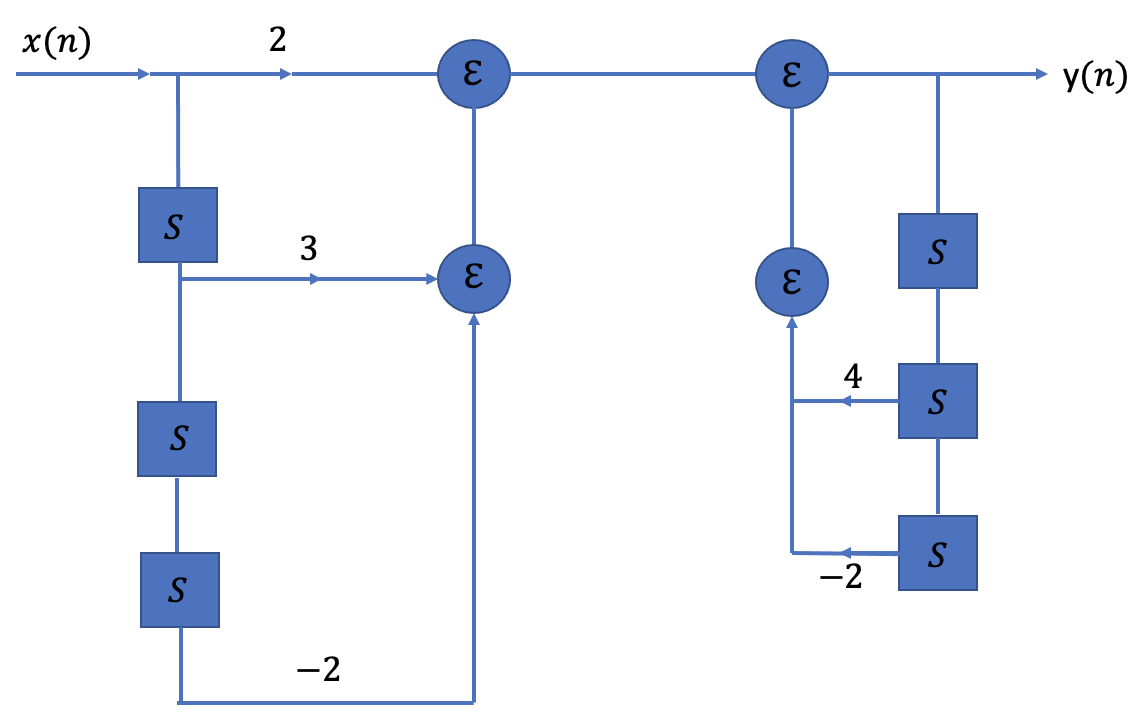
\includegraphics[scale=.29]{1.png}
\centering
\end{figure}
\end{itemize}
\newpage
\section*{\textbf{Question 3 (30 points): The systems given in Fig. 2 are equivalent systems.}}
\begin{itemize}
\item[(a)] (15 Pts.) Find $p_0$, $p_1$ for the system on the right side. ($p_0 > p_1$)
\item[(b)] (b) (15 Pts.) If the system was at rest, find y[5] for x[n] = $\delta$[n].
\\ \\
Left side system 1 and right side system 2.
\\ \\
System 1:
\begin{align*}
Part1:\\
w(n) = x(n) + p_0 \cdot w(n-1)\\
w(n) = p_0\cdot w(n-1) = x(n)\\
w(z) = \frac{x(z)}{1-p_0 z^{-1}}
\end{align*}
\begin{align*}
Part2:\\
y(z) = \frac{w(z)}{1-p_1z^{-1}}\\
y(z) =\frac{x(t)}{(1-p_0z^{-1})(1-p_1z^{-1}}\\
y(z) = \frac{x(z)}{1-(p_0+p_1)z^{-1} + p_0p_1z^{-2}}
\end{align*}
System 2:
\begin{align*}
y(n) = x(n) +0.6y(n-1) + 0.25y(n-2)\\
\Rightarrow y(n) = 0.6y(n-1) - 0.25y(n-2) = x(n)
\end{align*}
z transform,
\begin{align*}
y(z) -0.6 z^{-1}y(z) - 0.25z^{-2}y(z) = x(z)\\
y(z)(1 -0.6z^{-1} - 0.25z^{-2}) = x(z)\\
y(z) = \frac{x(z)}{1-0.6z^{-1}-0.25z^{-2}}
\end{align*}
\\ \\
\begin{align*}
p_0 + p_1 = 0.6\\
p_0\cdot p_1 = -0.25\\
p_0 = \frac{-0.25}{p_1}\\
p_1 = \frac{-0.25}{p_0}
\end{align*}
\end{itemize}






























\end{document}